\documentclass{article}
\usepackage{hyperref}
\usepackage{Style}
\setcounter{MaxMatrixCols}{20}

\nocite{*} % Comentar si quiero citar
%\addbibresource{bibliografia.bib} % Quitar el comentado si quiero usar bibliografia

\begin{document}

\begin{minipage}{2.5cm}
    \includegraphics[width=2cm]{imagen_puc.jpg}
\end{minipage}
\begin{minipage}{14cm}
    {\sc Pontificia Universidad Católica de Chile\\
    Facultad de Matemáticas\\
    Departamento de Matemática\\
    Profesor: Mauricio Bustamante -- Estudiante: Benjamín Mateluna}
\end{minipage}
\vspace{1ex}

{\centerline{\bf Topología Algebraica - MAT2850}
\centerline{\bf Tarea 2}}
\centerline{\bf 07 de septiembre de 2025}

\section*{Problema 3}
\noindent Por simplicidad del argumento, denotaremos los morfismos $A_{i}\to A_{i+1}$ y 
$B_{i}\to B_{i+1}$ como $\partial$. Debido a que ambas secuencias son exactas, resulta que 
$\partial^{2}a=\partial\circ\partial (a)=0$. Veamos que $\kr{f_{3}}=0$. Sea $a\in\kr{f_{3}}$,
notemos que
\begin{equation*}
    0=\partial f_{3}(a)=f_{4}\partial(a)\hhtext{entonces}\partial a=0
\end{equation*}
Como $a\in\kr\partial$, existe $a'\in A_{2}$ tal que $\partial a'=a$, luego $\partial f_{2}(a')
=f_{3}\partial(a')=f_{3}(a)=0$. Por exactitud, existe $b'\in B_{1}$ tal que $\partial b'
=f_{2}(a')$, puesto que $f_{1}$ es isomorfismo, existe $a''\in A_{1}$ tal que $b'=f_{1}(a'')$, 
usando que los diagramas conmutan vemos que
\begin{equation*}
    a''=f^{-1}_{1}(b')\hhtext{entonces}\partial a''=\partial f^{-1}_{1}(b')=f^{-1}_{2}\partial(b')
\end{equation*}
recordemos que $\partial b'=f_{2}(a')$, es decir, $\partial a''=a'$, luego 
$0=\partial^{2}a''=\partial a'=a$.

\vspace{2mm}
\noindent Sea $b\in B_{3}$, consideramos $\partial b\in B_{4}$, entonces 
$f^{-1}_{4}(\partial b)\in A_{4}$, por conmutatividad del diagrama, se sigue que
$\partial f_{4}^{-1}(\partial b)=f_{5}^{-1}(\partial^{2}b)=0$, luego, por exactitud, existe
$a\in A_{3}$ tal que $\partial a=f_{4}^{-1}(\partial b)$. Observemos que,
\begin{equation*}
    \partial(f_{3}(a)-b)=\partial f_{3}(a)-\partial b=f_{4}\partial(a)-\partial b=0
\end{equation*}
Así, existe $b'\in B_{2}$ tal que $\partial b'=f_{3}(a)-b$, definimos 
$a'=f_{2}^{-1}(b')\in A_{2}$, de este modo,
\begin{equation*}
    f_{3}(a)-b=\partial b'=\partial f_{2}(a')=f_{3}(\partial a')
\end{equation*}
En resumen, $f_{3}(a-\partial a')=b$. Concluimos que $f_{3}$ es isomorfismo.

\section*{Problema 4}
\noindent Sea $\Omega$ una colección finita de $2-$simplices, decimos que $\Omega$ se pega bien si 
cumple lo siguiente
\begin{enumerate}
    \item Para todo $\sigma,\tau\in\Omega$ se tiene que $\sigma\cap\tau$ es vacío o una cara de 
    ambos simplices.
    \item Para todo $\sigma\in\Omega$, existe $\tau\in\Omega$ tal que $\sigma\cap\tau$ es un 
    $1-$simplice.
    \item Existe $\sigma\in\Omega$ tal que existe un único $\tau\in\Omega$ de modo que 
    $\sigma\cap\tau$ es un $1-$simplice. Además, se tiene que $\Omega\setminus\{\sigma\}$ se pega 
    bien o consiste de un solo elemento.
\end{enumerate}
\noindent\textbf{Observación:} Por la primera propiedad, a cada colección finita de 
$2-$simplices que se pega bien, le podemos asignar un complejo simplicial. Adicionalmente, se 
tiene que dicho complejo simplicial es conexo gracias a la segunda propiedad.

\vspace{2mm}
\begin{lema}
    Sea $\Omega$ una colección finita de $2-$simplices que se pega bien. Sea $K$ el complejo 
    simplicial asociado a $\Omega$, entonces $H_{0}(K)=\Z$ y es trivial en otro caso.
\end{lema}
\begin{proof}
    Procederemos por inducción sobre el número de $2-$simplices en la colección. Para $n=1$ ya
    esta probado. Supongamos que se cumple para $n-1$, por definición, existe $\sigma\in\Omega$ 
    tal que $\Omega\setminus\{\sigma\}$ se pega bien, sea $M$ el complejo simplicial asociado. Sea
    $N$ el complejo simplicial que consiste en las caras de $\sigma$.

    \vspace{1mm}
    Como $\Omega$ se pega bien, existe un único $2-$simplice $\tau\in\Omega$ tal que 
    $\sigma\cap\tau$ es un $1-$simplice, entonces $M\cap N=\{\mu:\mu\leq\sigma\cap\tau\}$, que 
    resulta ser conexo como complejo simplicial. Usando Mayer-Vietoris, para $i>1$, es directo
    que $H_{0}(K)=0$. Por otro lado, para $i=1$, se sigue que

    \vspace{2mm}
    \centerline{
        \xymatrix{
            0 \ar[r] & 0 \ar[r] & H_{1}(K) \ar[r] & \Z \ar[r]^-{\varphi} & \Z^{2}
        }
    }
    
    \vspace{1mm}
    Notemos que el generador en $M\cap N$ se mapea a un generador tanto en $M$ como en $N$, vía el
    morfismo inducido por la inclusión. Entonces, $\varphi=(1,1)$, lo que implica que 
    $H_{1}(K)=0$, ya que $\kr{\varphi}=0$, lo que concluye la demostración.
\end{proof}

\newpage
\vspace{2mm}
\noindent Asignamos el orden a los vértices tal que $i<i+1$. Usaremos $R$ para denotar a los 
anillos $\Z,\Z_{2}$ y $\Q$. El lema anterior es válido para $R$.
\begin{enumerate}
    \item\textbf{Definición:} Notemos que el complejo simplicial es conexo, dado que el argumento 
    presentado en el problema 5 es invariante del anillo utilizado, se sigue que 
    $H_{0}(K)\cong R$. Adicionalmente, $C_{i}=0$ para $i>2$, ya que no hay $i-$simplices. Basta 
    calcular $H_{i}(K)$ para $i=1,2$. Tenemos el complejo de cadenas,

    \vspace{2mm}
    \centerline{
        \xymatrix{
            0 \ar[r] & C_{2} \ar[r]^{\partial_{2}} & C_{1} \ar[r]^{\partial_{1}} & C_{0} \ar[r] 
            & 0
        }
    }

    \vspace{2mm}
    Para encontrar los grupos de homología basta calcular $\kr{\partial_{2}},\im{\partial_{2}}$ y
    $\ker{\partial_{1}}$. A cada vértice en $C_{0}(K)$ le asignamos el vector canónico como sigue 
    $i=e_{i+1}$. A cada $1-$simplice le asignamos un vector de la siguiente manera,
    \begin{equation*}
        \begin{array}{llll}
            \gen{0,1}=e_{1} & \gen{0,5}=e_{5} & \gen{1,5}=e_{9} & \gen{3,4}=e_{13} \\
            \gen{0,2}=e_{2} & \gen{1,2}=e_{6} & \gen{2,3}=e_{10} & \gen{3,5}=e_{14} \\
            \gen{0,3}=e_{3} & \gen{1,3}=e_{7} & \gen{2,4}=e_{11} & \gen{4,5}=e_{15} \\
            \gen{0,4}=e_{4} & \gen{1,4}=e_{8} & \gen{2,5}=e_{12}
        \end{array}
    \end{equation*}
    Luego, la acción de $\partial_{1}$ esta representado por la matriz
    \begin{equation*}
        \begin{pmatrix}
            -1 & -1 & -1 & -1 & -1 & 0 & 0 & 0 & 0 & 0 & 0 & 0 & 0 & 0 & 0 \\
            1 & 0 & 0 & 0 & 0 & -1 & -1 & -1 & -1 & 0 & 0 & 0 & 0 & 0 & 0 \\
            0 & 1 & 0 & 0 & 0 & 1 & 0 & 0 & 0 & -1 & -1 & -1 & 0 & 0 & 0 \\
            0 & 0 & 1 & 0 & 0 & 0 & 1 & 0 & 0 & 1 & 0 & 0 & -1 & -1 & 0 \\
            0 & 0 & 0 & 1 & 0 & 0 & 0 & 1 & 0 & 0 & 1 & 0 & 1 & 0 & -1 \\
            0 & 0 & 0 & 0 & 1 & 0 & 0 & 0 & 1 & 0 & 0 & 1 & 0 & 1 & 1
        \end{pmatrix}
    \end{equation*}
    Usando SAGE, se obtiene que $\kr{\partial_{1}}\cong R^{10}$. Queda estudiar el morfismo 
    $\partial_{2}$. Realizamos la siguiente identificación
    \begin{equation*}
        \begin{array}{lll}
            \gen{0,1,3}=e_{1} & \gen{0,2,4}=e_{4} & \gen{1,2,5}=e_{7} \\
            \gen{0,2,3}=e_{2} & \gen{0,4,5}=e_{5} & \gen{1,3,4}=e_{8} \\
            \gen{0,1,5}=e_{3} & \gen{1,2,4}=e_{6} & \gen{2,3,5}=e_{9} \\
            & \gen{3,4,5}=e_{10}
        \end{array}
    \end{equation*}
    Junto con la identificación de los generadores de $C_{1}(K)$, el morfismo $\partial_{2}$ está
    representado por la matriz
    \begin{equation*}
        \begin{pmatrix}
            1 & 0 & 1 & 0 & 0 & 0 & 0 & 0 & 0 & 0 \\
            0 & 1 & 0 & 1 & 0 & 0 & 0 & 0 & 0 & 0 \\
            -1 & -1 & 0 & 0 & 0 & 0 & 0 & 0 & 0 & 0 \\
            0 & 0 & 0 & -1 & 1 & 0 & 0 & 0 & 0 & 0 \\
            0 & 0 & -1 & 0 & -1 & 0 & 0 & 0 & 0 & 0 \\
            0 & 0 & 0 & 0 & 0 & 1 & 1 & 0 & 0 & 0 \\
            1 & 0 & 0 & 0 & 0 & 0 & 0 & 1 & 0 & 0 \\
            0 & 0 & 0 & 0 & 0 & -1 & 0 & -1 & 0 & 0 \\
            0 & 0 & 1 & 0 & 0 & 0 & -1 & 0 & 0 & 0 \\
            0 & 1 & 0 & 0 & 0 & 0 & 0 & 0 & 1 & 0 \\
            0 & 0 & 0 & 1 & 0 & 1 & 0 & 0 & 0 & 0 \\
            0 & 0 & 0 & 0 & 0 & 0 & 1 & 0 & -1 & 0 \\
            0 & 0 & 0 & 0 & 0 & 0 & 0 & 1 & 0 & 1 \\
            0 & 0 & 0 & 0 & 0 & 0 & 0 & 0 & 1 & -1 \\
            0 & 0 & 0 & 0 & 1 & 0 & 0 & 0 & 0 & 1
        \end{pmatrix}
    \end{equation*}
    Nuevamente, usando SAGE, se obtiene que $\kr{\partial_{2}}=0$ si $R=\Z,\Q$, pero en $\Z^{2}$ 
    se tiene que $\kr{\partial_{2}}=\Z_{2}$. Además, $\im{\partial_{2}}=\Z_{2}^{9}$ cuando 
    $R=\Z_{2}$, mientras que para $\Z$ tenemos que $\im{\partial_{2}}=2\Z\oplus\Z^{9}$ y para 
    $\Q$, $\im{\partial_{2}}=\Q^{10}$. Entonces,
    \begin{equation*}
        H_{i}(K;\Z_{2})=\begin{cases}
            \Z_{2} &\quad\text{si }i=0,1,2 \\
            0 &\quad\text{si }i\neq0,1,2
        \end{cases}
        \hspace{1cm}
        H_{i}(K;\Z)=\begin{cases}
            \Z & \quad\text{si }i=0 \\
            \Z_{2} & \quad\text{si }i=1 \\
            0 & \quad\text{si }i\neq0,1
        \end{cases}
        \hspace{1cm}
        H_{i}(K;\Q)=\begin{cases}
            \Q & \quad\text{si }i=0 \\
            0 & \quad\text{si }i\neq0
        \end{cases}
    \end{equation*}

    \newpage
    \item\textbf{Mayer-Vietoris:} Consideramos los siguientes subcomplejos simpliciales,
    \begin{center}
        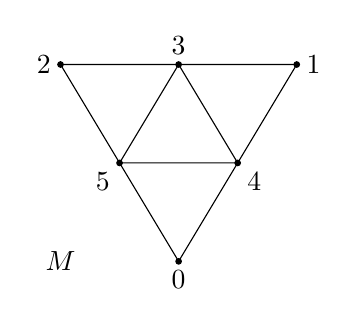
\begin{tikzpicture}[scale=1] %Subcomplejo M
            \coordinate (A) at (-1.5,1.5);
            \coordinate (B) at (1.5,1.5);
            \coordinate (C) at (0,-1);

            \coordinate (D) at (0,1.5);
            \coordinate (E) at (-0.75,0.25);
            \coordinate (F) at (0.75,0.25);

            \draw (A) -- (B) -- (C) -- cycle;
            \draw (D) -- (E) -- (F) -- cycle;

            \filldraw (-1.5,-1) node{$M$};
            
            \filldraw (A) circle (1pt) node[anchor=east]{$2$};
            \filldraw (B) circle (1pt) node[anchor=west]{$1$};
            \filldraw (C) circle (1pt) node[anchor=north]{$0$};

            \filldraw (D) circle (1pt) node[anchor=south]{$3$};
            \filldraw (E) circle (1pt) node[anchor=north east]{$5$};
            \filldraw (F) circle (1pt) node[anchor=north west]{$4$};
        \end{tikzpicture}
        %
        \hspace{1cm}
        %
        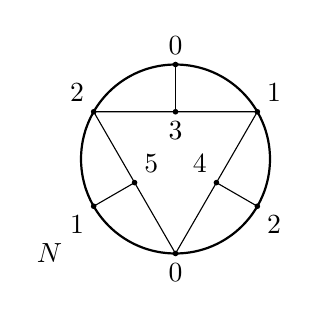
\begin{tikzpicture}[scale=0.8] %Subcomplejo N
            \filldraw[color=black, fill=white, thick] circle (1.5);

            \coordinate (A) at ({-3*sqrt(3)/4},{3/4});
            \coordinate (B) at ({3*sqrt(3)/4},{3/4});
            \coordinate (C) at (0,-1.5);

            \coordinate (D) at (0,1.5);
            \coordinate (E) at ({-3*sqrt(3)/4},{-3/4});
            \coordinate (F) at ({3*sqrt(3)/4},{-3/4});

            \coordinate (G) at (0,{3/4});
            \coordinate (H) at ({-3*sqrt(3)/8},{-3/8});
            \coordinate (I) at ({3*sqrt(3)/8},{-3/8});

            \draw (A) -- (B) -- (C) -- cycle;
            
            \draw (D) -- (G);
            \draw (E) -- (H);
            \draw (F) -- (I);

            \filldraw (-2,-1.5) node{$N$};

            \filldraw (A) circle (1pt) node[anchor=south east]{$2$};
            \filldraw (B) circle (1pt) node[anchor=south west]{$1$};
            \filldraw (C) circle (1pt) node[anchor=north]{$0$};

            \filldraw (D) circle (1pt) node[anchor=south]{$0$};
            \filldraw (E) circle (1pt) node[anchor=north east]{$1$};
            \filldraw (F) circle (1pt) node[anchor=north west]{$2$};

            \filldraw (G) circle (1pt) node[anchor=north]{$3$};
            \filldraw (H) circle (1pt) node[anchor=south west]{$5$};
            \filldraw (I) circle (1pt) node[anchor=south east]{$4$};
        \end{tikzpicture}
    \end{center}
    Por el lema, se tiene que $H_{0}(M)=R$ y es trivial en otro caso, además, vemos que 
    $H_{i}(M\cap N)=R$ para $i=0,1$ y es cero en otro caso. Por otro lado, para $N$, consideramos 
    la subdivisión en complejos simpliciales como sigue,
    \begin{center}
        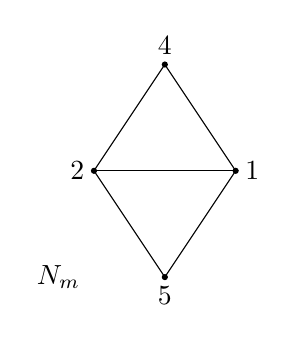
\begin{tikzpicture}[scale=0.9] %Primer subcomplejo de N
            \coordinate (A) at (0,1.5);
            \coordinate (B) at (-1,0);
            \coordinate (C) at (0,-1.5);
            \coordinate (D) at (1,0);

            \draw (A) -- (B) -- (C) -- (D) -- cycle;
            \draw (B) -- (D);

            \filldraw (A) circle (1pt) node[anchor=south]{$4$};
            \filldraw (B) circle (1pt) node[anchor=east]{$2$};
            \filldraw (C) circle (1pt) node[anchor=north]{$5$};
            \filldraw (D) circle (1pt) node[anchor=west]{$1$};

            \filldraw (-1.5,-1.5) node{$N_{m}$};
        \end{tikzpicture}
        %
        \hspace{1cm}
        %
        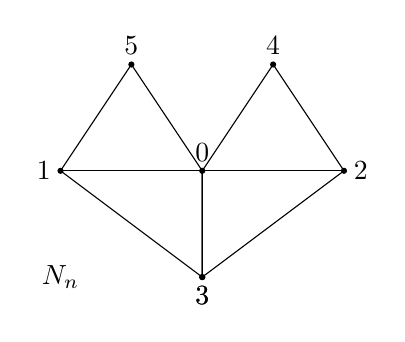
\begin{tikzpicture}[scale=0.9] %Segundo subcomplejo de N
            \coordinate (A) at (-2,1.5);
            \coordinate (B) at (-3,0);
            \coordinate (C) at (-1,-1.5);
            \coordinate (D) at (-1,0);

            \draw (A) -- (B) -- (C) -- (D) -- cycle;
            \draw (B) -- (D);

            \filldraw (A) circle (1pt) node[anchor=south]{$5$};
            \filldraw (B) circle (1pt) node[anchor=east]{$1$};
            \filldraw (C) circle (1pt) node[anchor=north]{$3$};

            \coordinate (A) at (0,1.5);
            \coordinate (B) at (-1,0);
            \coordinate (C) at (-1,-1.5);
            \coordinate (D) at (1,0);

            \draw (A) -- (B) -- (C) -- (D) -- cycle;
            \draw (B) -- (D);

            \filldraw (A) circle (1pt) node[anchor=south]{$4$};
            \filldraw (B) circle (1pt) node[anchor=south]{$0$};
            \filldraw (C) circle (1pt) node[anchor=north]{$3$};
            \filldraw (D) circle (1pt) node[anchor=west]{$2$};

            \filldraw (-3,-1.5) node{$N_{n}$};
        \end{tikzpicture}
    \end{center}
    Nuevamente, por el lema, se sigue que $H_{0}(N_{m})=H_{0}(N_{n})=R$ y es trivial en otro caso.
    Por otro lado, $H_{0}(N_{m}\cap N_{n})$ consiste en la unión disjunta de dos $1-$simplices,
    luego, $H_{0}(N_{m}\cap N_{n})=R^{2}$ y es cero en otro caso. Entonces, usando Mayer-Vietoris
    resulta que

    \vspace{2mm}
    \centerline{
        \xymatrix{
            0 \ar[r] & 0 \ar[r] & H_{i}(N) \ar[r] & 0\\
        }
    }
    \vspace{1mm}
    donde $i>1$. Por lo tanto, $H_{i}(N)=0$ cuando $i>1$. Veamos cuando $i=1$, se tiene la 
    siguiente secuencia exacta

    \vspace{2mm}
    \centerline{
        \xymatrix{
            0 \ar[r] & 0 \ar[r] & H_{1}(N) \ar[r] & R^{2} \ar[r]^{\varphi} & R^{2}
        }
    }
    \vspace{1mm}
    Como $N_{m}\cap N_{n}$ posee dos componentes conexas, es generado por dos elementos, por ende,
    cada generador se mapea a un generador tanto en $H_{0}(N_{m})$ como en $H_{0}(N_{n})$ vía el
    morfismo inducido por la inclusión, lo que implica que
    \begin{equation*}
        \varphi=\begin{pmatrix}
            1 & 1 \\ 1 & 1
        \end{pmatrix}
    \end{equation*}
    Por exactitud, $H_{1}(N)=R$, puesto que $\kr{\varphi}\cong R$. Para $i=0$ sabemos que el 
    complejo es conexo, entonces $H_{0}(N)= R$. Volviendo al Mayer-Vietoris original, tenemos que

    \vspace{2mm}
    \centerline{
        \xymatrix{
            0 \ar[r] & 0 \ar[r] & H_{2}(K) \ar[r] & R \ar[r]^-{\psi} 
            & R \ar[r]^-{\phi} & H_{1}(K)
            \ar `[ld] `[l] `[llllld] `[l] [dllll] \\
            & R \ar[r]^{\varphi} & R^{2} \ar[r] & H_{0}(K) \ar[r] & 0
        }
    }
    \vspace{1mm}
    Notemos que el mapeo $H_{1}(M\cap N)\to H_{1}(M)$ es trivial, mientras que el generador en 
    $H_{1}(M\cap N)$, a saber,
    \begin{equation*}
        \tau=\gen{1,4}-\gen{0,4}+\gen{0,5}+\gen{2,5}-\gen{2,3}-\gen{1,3}
    \end{equation*}
    se mapea dos veces al generador en $H_{1}(N)$ que es $\sigma=\gen{0,1}+\gen{1,2}-\gen{0,2}$.
    En efecto, notemos que
    \begin{equation*}
        \partial_{2}(\gen{0,2,3}+\gen{0,1,3}-\gen{0,2,4}+\gen{0,1,5}+\gen{1,2,5}-\gen{0,2,3})=
        2\sigma-\tau
    \end{equation*}
    De este modo, $\kr{\psi}=0$ para $\Z$ y $\Q$, mientras que $\kr{\psi}=\Z_{2}$ para $\Z_{2}$.
    Luego, $\im{\psi}=2\Z$, $\im{\psi}=\Q$ y finalmente $\im{\psi}=0$ cuando vemos los 
    coeficientes en $\Z,\Q$ y $\Z_{2}$ respectivamente. Por otro lado, por la misma razón que 
    antes, $\varphi=(1,1)$, es decir, $\kr{\varphi}=0$ para $R$ y entonces $\phi$ es sobreyectivo. 
    Por primer teorema de isomorfismo y exactitud, concluimos que
    \begin{equation*}
        H_{i}(K;\Z_{2})=\begin{cases}
            \Z_{2} &\quad\text{si }i=0,1,2 \\
            0 &\quad\text{si }i\neq0,1,2
        \end{cases}
        \hspace{1cm}
        H_{i}(K;\Z)=\begin{cases}
            \Z & \quad\text{si }i=0 \\
            \Z_{2} & \quad\text{si }i=1 \\
            0 & \quad\text{si }i\neq0,1
        \end{cases}
        \hspace{1cm}
        H_{i}(K;\Q)=\begin{cases}
            \Q & \quad\text{si }i=0 \\
            0 & \quad\text{si }i\neq0
        \end{cases}
    \end{equation*}
\end{enumerate}

\section*{Problema 5}
\noindent Sea $K$ un complejo simplicial finito y sean $v,w\in V_{K}$, decimos que $v\sim_{p}w$ si
y solo si $v$ esta conectado a $w$ ó $v=w$, es decir, si existe una sucesión de $1-$simplices
$\gen{w_{0},w_{1}},\cdots,\gen{w_{k-1},w_{k}}$ tales que $w_{0}=v$ y $w_{k}=w$.

\vspace{1mm}
\noindent Por definición resulta que $x\sim_{p}x$, además, notemos que si $v\sim_{p}w$ entonces 
$w\sim_{p}v$ basta tomar $\omega_{i}:=w_{k-i}$. Por otro lado, si $v\sim_{p}w$ y $w\sim_{p}u$, 
entonces la sucesión
\begin{equation*}
    \gen{w_{0},w_{1}},\cdots,\gen{w_{k-1},w_{k}},\gen{\omega_{0},\omega_{1}},\cdots,
    \gen{\omega_{j-1},\omega_{j}}
\end{equation*}
donde $w_{0}=v$, $w_{k}=w$, $\omega_{0}=w$ y $\omega_{j}=u$ es una sucesión que conecta $v$ con 
$u$, en otras palabras, $v\sim_{p}u$.

\vspace{2mm}
\begin{dfn}[Componente Conexa]
    Sea $K$ un complejo simplicial finito y $v\in V_{K}$, definimos su componente conexa
    como
    \begin{equation*}
        [v]_{c}:=\{\sigma\in K:\sigma=\gen{v_{0},v_{1},\cdots,v_{r}}\hhtext{y}v\sim_{p}v_{i}\}
    \end{equation*}
\end{dfn}

\noindent\textbf{Observación:} Si $[v]_{c}=K$, entonces el complejo simplicial es conexo. Sea 
$w\in V_{K}$ tal que $w\in[v]_{c}$, entonces $v\sim_{p}w$. Luego, dado $\sigma
=\gen{v_{0},\cdots,v_{r}}\in[w]_{c}$ se tiene que $v\sim_{p}v_{i}$, se sigue que 
$[w]_{c}\subseteq[v]_{c}$, de manera similar obtenemos que $[v]_{c}\subseteq[w]_{c}$. Por lo tanto
$[w]_{c}=[v]_{c}$.

\vspace{1mm}
\noindent Veamos que dado $v\in V_{K}$, se tiene que $[v]_{c}$ es un subcomplejo simplicial de 
$K$. En efecto, sea $\sigma\in[v]_{c}$ y $\tau\leq\sigma$, si $v_{i}$ es un vértice de $\tau$ 
entonces es vértice de $\sigma$, luego $v\sim_{p}v_{i}$, lo que implica que $\tau\in[v]_{c}$. La
segunda propiedad se cumple trivialmente. Por lo tanto, una componente conexa es un subcomplejo 
simplicial conexo de $K$ y la unión de dos componentes conexas también es subcomplejo simplicial, 
puesto que un simplice esta en una componente conexa o en la otra, pero no en ambas.

\vspace{1mm}
\noindent Como $\sim_{p}$ es una relación de equivalencia, particiona el conjunto de vértices,
junto con lo anterior hemos probado que las componentes conexas particionan al complejo 
simplicial.

\vspace{2mm}
\noindent Debemos probar lo siguiente:
\begin{enumerate}
    \item\textbf{Si $K$ es conexo, entonces $\abs{K}$ arcoconexo}. Sean $x,y\in\abs{K}$, 
    existen $\sigma_{x},\sigma_{y}\in K$ tales que $x\in\sigma_{x}$ e $y\in\sigma_{y}$, sean 
    $v_{x}\in\sigma_{x}$ y $v_{y}\in\sigma_{y}$ vértices de $K$. Existe una sucesión
    \begin{equation*}
        \gen{w_{0},w_{1}},\cdots,\gen{w_{k-1},w_{k}}
    \end{equation*}
    tal que $w_{0}=v_{x}$ y $w_{k}=v_{y}$, consideramos la función $f_{i}:[0,1]\to\abs{K}$ dada 
    por $f_{i}(t):=(1-t)w_{i}+tw_{i+1}$ que esta bien definida por que $\gen{w_{i},w_{i+1}}$ es 
    convexo y es continua. Del mismo modo, como $\sigma_{x}$ es convexo, la función 
    $f_{x}:[0,1]\to\abs{K}$ dada por $f_{x}(t):=(1-t)x+tv_{x}$ esta bien definida. De manera
    análoga, definimos $f_{y}$, pero $f_{y}(0)=v_{y}$ y $f_{y}(1)=y$. Luego,
    \begin{equation*}
        f:=f_{x}\sbullet f_{0}\sbullet f_{1}\sbullet\cdots\sbullet f_{k-1}\sbullet f_{y}
    \end{equation*}
    donde $\sbullet$ es la operación de concatenación. Es una función continua, por lema del 
    pegamiento, tal que $f(0)=x$ y $f(1)=y$.
    
    \vspace{1mm}
    Concluimos que $\abs{K}$ es arcoconexo.
    
    \item\textbf{Probar que $H_{0}(K)\cong\Z^{\text{\#componentes conexas}}$}. Como $K$ es 
    finito, hay finitas componentes conexas, procederemos por inducción en el número de 
    componentes conexas.

    \vspace{1mm}
    Supongamos que $K$ tiene una componente conexa, entonces $K$ es conexo. Dado $v\in V_{K}$, 
    basta probar que $[v]=[w]$ en $H_{0}(K)$ para todo $w\in V_{K}$. Como $K$ es conexo, existe
    una sucesión
    \begin{equation*}
        \gen{w_{0},w_{1}},\cdots,\gen{w_{k-1},w_{k}}
    \end{equation*}
    tal que $w_{0}=v$ y $w_{k}=w$, entonces
    \begin{equation*}
        \partial\left(\sum_{i=0}^{k-1}\gen{w_{i},w_{i+1}}\right)
        =\sum_{i=0}^{k-1}\partial\gen{w_{i},w_{i+1}}=\sum_{i=0}^{k-1}w_{i+1}-w_{i}=w_{k}-w_{0}=w-v
    \end{equation*}
    luego $w-v\in\im{\partial}$. Entonces $H_{0}(K)\cong\Z$.

    \vspace{1mm}
    Sea $n$ el número de componentes conexas. Sean $M_{i}$ las componentes conexas de $K$, 
    consideramos los subcomplejos simpliciales
    \begin{equation*}
        M=M_{n} \hhtext{y} N=\bigcup_{i=1}^{n-1}M_{i}
    \end{equation*}
    Por Mayer-Vietoris, se tiene la siguiente secuencia exacta
    
    \vspace{2mm}
    \centerline{
        \xymatrix{
            0 \ar[r] & H_{0}(M)\oplus H_{0}(N) \ar[r] & H_{0}(K) \ar[r] & 0
        }
    }
    entonces
    \begin{equation*}
        H_{0}(K)\cong H_{0}(M)\oplus H_{0}(N)\cong\Z\oplus\Z^{n-1}\cong\Z^{n}
    \end{equation*}
\end{enumerate}

%\printbibliography % Quitar el comentado si quiero usar bibliografia

\end{document}
